\documentclass[11pt, a4paper]{article}

% --- Packages ---
\usepackage[utf8]{inputenc}
\usepackage[T1]{fontenc}
\usepackage[spanish, es-tabla]{babel}
\usepackage{amsmath, amssymb, amsthm}
\usepackage{graphicx}
\usepackage{booktabs}
\usepackage{xcolor}
\usepackage[colorlinks=true, linkcolor=blue!60!black, urlcolor=blue!60!black, citecolor=blue!60!black]{hyperref}
\usepackage[margin=2.5cm]{geometry}
\usepackage{fancyhdr}
\usepackage{titlesec}
\usepackage{caption}
\usepackage{subcaption}
\usepackage{array}
\usepackage{tabularx}
\usepackage{enumitem}
\usepackage{listings}
\usepackage{tcolorbox}
\usepackage{xurl}

% --- Style ---
\pagestyle{fancy}
\fancyhf{}
\fancyhead[L]{\small Reporte Etapa 2 - Mamba Exoplanet}
\fancyhead[R]{\small ITCR · IA · 2026-I}
\fancyfoot[C]{\thepage}
\renewcommand{\headrulewidth}{0.4pt}

\titleformat{\section}{\Large\bfseries\color{blue!50!black}}{\thesection.}{0.5em}{}
\titleformat{\subsection}{\large\bfseries}{\thesubsection.}{0.5em}{}

\captionsetup{font=small, labelfont=bf}
\setlength{\parskip}{0.5em}
\setlength{\parindent}{0pt}

\lstset{
    basicstyle=\ttfamily\small,
    breaklines=true,
    frame=single,
    framesep=4pt,
    backgroundcolor=\color{gray!10},
    rulecolor=\color{gray!50},
    showstringspaces=false,
}

\newtcolorbox{keybox}[1][]{
    colback=blue!5!white,
    colframe=blue!50!black,
    boxrule=0.5pt,
    arc=2pt,
    left=8pt, right=8pt, top=6pt, bottom=6pt,
    #1
}

% --- Title ---
\title{
    \vspace{-1.5cm}
    \textbf{Reporte Técnico - Etapa 2}\\[0.3em]
    \large Modelos de Espacio de Estados (Mamba) para Detección\\ de Exoplanetas en Curvas de Luz de TESS
}
\author{
    José Fabián Zumbado Ruiz \and Jeremmy Aguilar Villanueva\\
    \small Curso: Inteligencia Artificial - Prof. Kenneth Obando Rodríguez\\
    \small Escuela de Ingeniería en Computación, Instituto Tecnológico de Costa Rica
}
\date{Semestre I - 2026 (cierre semana 10)}

\begin{document}

\maketitle
\thispagestyle{fancy}

% --- Abstract / Resumen ejecutivo ---
\section*{Resumen ejecutivo}

Este reporte cubre la \textbf{Etapa 2} del proyecto: modelado, entrenamiento, optimización, explicabilidad (XAI) y evaluación rigurosa de modelos para vetting de candidatos a exoplaneta del catálogo TOI de TESS. Implementamos una \textbf{escalera de seis modelos} que aíslan, una a una, las variables de diseño relevantes (features físicas vs. fotometría cruda, vista global vs. local, CNN vs. SSM, single-branch vs. dual-branch) y los comparamos sobre un \textbf{test sellado} evaluado una sola vez por modelo.

\begin{keybox}
\textbf{Hallazgo principal:} Mamba single-view aplasta a todos los baselines (test AUC-ROC \textbf{0.806} con ensemble de 5 semillas; \textbf{0.810} con la mejor semilla individual), superando al CNN single-branch por \textbf{+20 puntos porcentuales} y a la reproducción fiel de AstroNet multibranch por \textbf{+9 puntos}. Esto representa \textbf{7 veces} el umbral ``Excelente'' ($\geq +3$ pp) declarado en la propuesta original.
\end{keybox}

Hallazgos secundarios paper-worthy:
\begin{enumerate}[leftmargin=*, topsep=0pt]
    \item \textbf{AstroNet multibranch} (1.34\,M parámetros) con vista local supera al CNN single-branch en \textbf{+11 pp} - el phase-folding del tránsito aporta señal real al CNN.
    \item Una fusión naive late-concat de Mamba + CNN local (\textbf{ExoMamba V1}) \textbf{colapsa por debajo del azar} (AUC 0.46) - ablation negativa que demuestra que la dirección de fusión global+local con SSM exige operadores no-triviales.
\end{enumerate}

\begin{table}[h]
\centering
\small
\begin{tabular}{lrrr}
\toprule
\textbf{Métrica} & Aceptable & Excelente & \textbf{Mamba ensemble} \\
\midrule
Mejora AUC vs.\ CNN & $\geq +1$ pp & $\geq +3$ pp & \textbf{+20 pp} \checkmark \\
Recall (clase CP) & $\geq 0.80$ & $\geq 0.90$ & \textbf{0.824} \checkmark \\
AUC-ROC absoluto & $\geq 0.88$ & $\geq 0.93$ & 0.806 (esperable con $N=1576$) \\
\bottomrule
\end{tabular}
\caption{Umbrales de la propuesta original vs. resultados Mamba ensemble.}
\end{table}

\tableofcontents
\newpage

% =============================================================================
\section{Contexto y problema}

\subsection{Detección vs.\ vetting de exoplanetas}

La misión \textbf{TESS} (Transiting Exoplanet Survey Satellite, NASA, 2018+) observa más de 200,000 estrellas con cadencia de 2 minutos. Cada estrella produce una serie temporal de $\sim 18{,}000$ mediciones de brillo por sector de $\sim 27$ días. Las señales de tránsito planetario aparecen como \textbf{caídas periódicas y simétricas} de $\sim 0.01\!-\!1\%$ del flujo, frecuentemente confundibles con binarias eclipsantes y artefactos instrumentales.

Nuestro problema \textbf{NO es detección desde cero} (eso lo hace la pipeline de NASA con BLS). Es \textbf{vetting}: clasificar candidatos ya detectados (TOIs --- TESS Objects of Interest) como planeta confirmado (CP) o falso positivo (FP). Para cada TIC tenemos:

\begin{itemize}[leftmargin=*, topsep=0pt]
    \item La \textbf{curva de luz cruda} ($\sim 18{,}000$ puntos de flujo PDCSAP normalizado).
    \item \textbf{Metadatos del catálogo TOI} disponibles porque el TOI ya existe: período orbital $P$, profundidad del tránsito, época de tránsito $T_0$, magnitud estelar $T_{\text{mag}}$, duración $D$.
\end{itemize}

Esto hace \textbf{legítimo} usar el catálogo como input (no es data leakage en este setting), siguiendo la práctica establecida por ExoMiner y AstroNet.

\begin{figure}[h]
\centering
\includegraphics[width=0.6\textwidth]{../public/observation_sector.jpg}
\caption{Sector típico de TESS (NASA/MIT). Cada sector cubre $\sim 27$ días continuos con cadencia de 2 minutos.}
\end{figure}

\subsection{Métricas objetivo}

Clasificación binaria desbalanceada (1576 etiquetados: 603 CP + 973 FP tras filtrado de calidad, $\sim 1\!:\!1.6$). Métricas centradas en la clase positiva:

$$
\text{Recall} = \frac{TP}{TP+FN}, \quad \text{Precision} = \frac{TP}{TP+FP}, \quad F_1 = \frac{2 \cdot P \cdot R}{P + R}
$$

Y métricas globales independientes del umbral:

$$
\text{AUC-ROC} = P(\hat{p}_+ > \hat{p}_-)
$$

(probabilidad de que un positivo aleatorio se rankee por encima de un negativo aleatorio).

$$
\text{Brier} = \frac{1}{N}\sum_{i=1}^N (\hat{p}_i - y_i)^2 \quad \text{(calibración cuadrática)}
$$

La \textbf{accuracy} se descarta a propósito: con ratio FP:CP $\approx 2.1\!:\!1$, predecir siempre ``FP'' da accuracy $\approx 0.68$ sin aprender nada.

% =============================================================================
\section{Baselines y modelos implementados}

Implementamos seis modelos que forman una \textbf{escalera controlada} donde cada escalón agrega exactamente una variable de diseño:

\begin{table}[h]
\centering
\small
\begin{tabular}{clcccrr}
\toprule
\# & Modelo & Global & Local & Catálogo & Params & Tier \\
\midrule
1 & Random estratificado & --- & --- & --- & 0 & 1 \\
2 & Catalog Logistic Regression & --- & --- & \checkmark & $\sim$10 & 1 \\
3 & CNN single-branch (AstroNet-single) & \checkmark & --- & --- & 62{,}881 & 1 \\
4 & \textbf{Mamba single-view (principal)} & \checkmark & --- & --- & 131{,}393 & 1 \\
5 & ExoMamba V1 (Mamba+local, late-concat) & \checkmark & \checkmark & --- & $\sim$153K & 2 \\
6 & AstroNet multibranch (reproducción fiel) & \checkmark & \checkmark & --- & 1{,}338{,}081 & 2 \\
\bottomrule
\end{tabular}
\caption{Escalera de modelos: cada fila agrega exactamente una variable de diseño.}
\end{table}

Esta escalera satisface holgadamente el requisito ``$\geq 2$ baselines razonables'' del rubric (Excelente, 10\%) y permite \textbf{atribuir cada delta de AUC a un componente concreto} en la discusión.

\subsection{Baseline 1: Random estratificado}

Predice según el prior de clase: $P(y=1) = n_{CP}/(n_{CP}+n_{FP}) \approx 0.32$. Sin entrenamiento, sirve de \textbf{piso mínimo} (AUC esperada $= 0.5$).

\subsection{Baseline 2: Catalog Logistic Regression}

\textbf{¿Qué es Logistic Regression?} El modelo más simple de clasificación binaria. Combina linealmente las features y aplica la función sigmoide para producir una probabilidad:

$$
P(y=1 \mid \mathbf{x}) = \sigma(\mathbf{w}^\top \mathbf{x} + b), \qquad \sigma(z) = \frac{1}{1 + e^{-z}}
$$

donde $\mathbf{x} \in \mathbb{R}^3$ contiene las features del catálogo TOI: $[P_{\text{orb}}, \text{profundidad tránsito}, T_{\text{mag}}]$. Los pesos $\mathbf{w}$ se aprenden minimizando la \textbf{Binary Cross-Entropy} (BCE) con \texttt{class\_weight="balanced"}:

$$
\mathcal{L}_{\text{BCE}} = -\frac{1}{N}\sum_{i=1}^N \left[ w_+ \, y_i \log(\hat{p}_i) + (1 - y_i) \log(1 - \hat{p}_i) \right], \quad w_+ = \frac{n_{\text{neg}}}{n_{\text{pos}}}
$$

Standarización de features con \texttt{StandardScaler} fiteado \textbf{solo en train} (defensa contra data leakage).

Este baseline responde una pregunta fundamental: \textbf{¿basta con la metadata del catálogo para discriminar CP de FP, o hace falta la curva?} Si la metadata sola ya separa las clases, todos nuestros CNN/SSM están sobre-ingenierizados.

\subsection{Baseline 3: CNN 1D single-branch}

CNN inspirada en \textbf{AstroNet} (Shallue \& Vanderburg, 2018) restringida a la vista global única. Cuatro bloques convolucionales con BatchNorm + ReLU + MaxPool:

\begin{lstlisting}[basicstyle=\ttfamily\footnotesize]
Conv1d(1->16, k=5)   -> BN -> ReLU -> MaxPool(2)   # (B, 16, 9000)
Conv1d(16->32, k=5)  -> BN -> ReLU -> MaxPool(2)   # (B, 32, 4500)
Conv1d(32->64, k=5)  -> BN -> ReLU -> MaxPool(2)   # (B, 64, 2250)
Conv1d(64->128, k=5) -> BN -> ReLU -> MaxPool(2)   # (B, 128, 1125)
AdaptiveAvgPool1d(1) -> Linear(128->64) -> ReLU -> Dropout(0.3) -> Linear(64->1)
\end{lstlisting}

\textbf{¿Qué hace una convolución 1D?} Aplica un filtro deslizante de longitud $K$ sobre la secuencia:

$$
(x \star w)_t = \sum_{k=0}^{K-1} x_{t+k} \cdot w_k
$$

El filtro aprendido captura \textbf{patrones locales} (e.g.\ una caída en forma de U típica de un tránsito) en una vecindad de $K$ puntos. Apilando capas con pooling, el campo receptivo crece geométricamente pero \textbf{nunca alcanza los 18,000 puntos completos} --- un CNN ve la curva como una colección de patches locales, no como un todo.

\subsection{Modelo principal: Mamba single-view}

\textbf{¿Qué hace Mamba diferente?} Mamba (Gu \& Dao, 2023) es una arquitectura basada en \textbf{Selective State Space Models} (SSM). En lugar de convolución local o atención cuadrática (Transformer), Mamba mantiene un \textbf{estado latente $h_t$} que se actualiza secuencialmente:

\begin{keybox}
$$
h_t = \bar{\mathbf{A}}_t \, h_{t-1} + \bar{\mathbf{B}}_t \, x_t, \qquad y_t = \mathbf{C}_t \, h_t
$$
donde $\bar{\mathbf{A}}, \bar{\mathbf{B}}, \mathbf{C}$ son matrices que \textbf{dependen del input} $x_t$ (eso es lo ``selective'').
\end{keybox}

Esto le permite a Mamba:

\begin{enumerate}[leftmargin=*, topsep=0pt]
    \item \textbf{Capturar dependencias a 18,000 pasos} en complejidad $O(L)$ --- un Transformer requeriría $O(L^2) = O(3.24 \times 10^8)$ operaciones por capa, inviable en una RTX 3050.
    \item \textbf{Ignorar selectivamente partes irrelevantes} de la secuencia (ruido instrumental, gaps por mala calidad) ajustando $\bar{\mathbf{B}}_t$ cerca de cero.
    \item \textbf{Acumular evidencia a largo plazo}: si hay 5 tránsitos espaciados cada 5 días en una curva de 27 días, Mamba puede integrar los 5 en el estado $h$, mientras que un CNN los procesa de forma independiente.
\end{enumerate}

Configuración (\texttt{mamba\_baseline.py}):

\begin{lstlisting}[basicstyle=\ttfamily\footnotesize]
Linear embed(1 -> d_model=64)
[Mamba block] x n_layers=4
    - d_state=16, d_conv=4, expand=2
    - LayerNorm + residual
GlobalAveragePool(L) -> (B, 64)
Linear(64 -> 1) -> logit
\end{lstlisting}

\textbf{131{,}393 parámetros entrenables}. Mixed precision (FP16) opcional (descartado en sanity y baseline final por estabilidad numérica), gradient clipping \texttt{max\_norm=1.0} (crítico --- sin clipping Mamba diverge con NaN sobre secuencias largas).

\subsection{Ablation Tier 2: ExoMamba V1 (Mamba + CNN local, late-concat)}

Modelo híbrido que \textbf{busca} complementar el modelado de largo plazo con detalle local fino:

\begin{lstlisting}[basicstyle=\ttfamily\footnotesize]
global_view  -> Mamba encoder    -> vector (B, 64)
local_view   -> CNN 3-bloques    -> vector (B, 64)
                concat           -> (B, 128)
                MLP(128->64->1)  -> logit
\end{lstlisting}

La vista local se construye por \textbf{phase-folding}:

$$
\phi(t) = \frac{(t - T_0) \bmod P}{P}, \qquad \text{ventana: } \left| \phi - 0.5 \right| \le 2.5 \cdot \frac{D}{P}
$$

Esto pliega las múltiples órbitas observadas en un solo tránsito promediado, ganando $\sqrt{N_{\text{órbitas}}}$ en SNR. Binneamos a 201 puntos uniformes y normalizamos por mediana propia. Ejemplos visuales en la Figura~\ref{fig:local_samples}.

\begin{figure}[h]
\centering
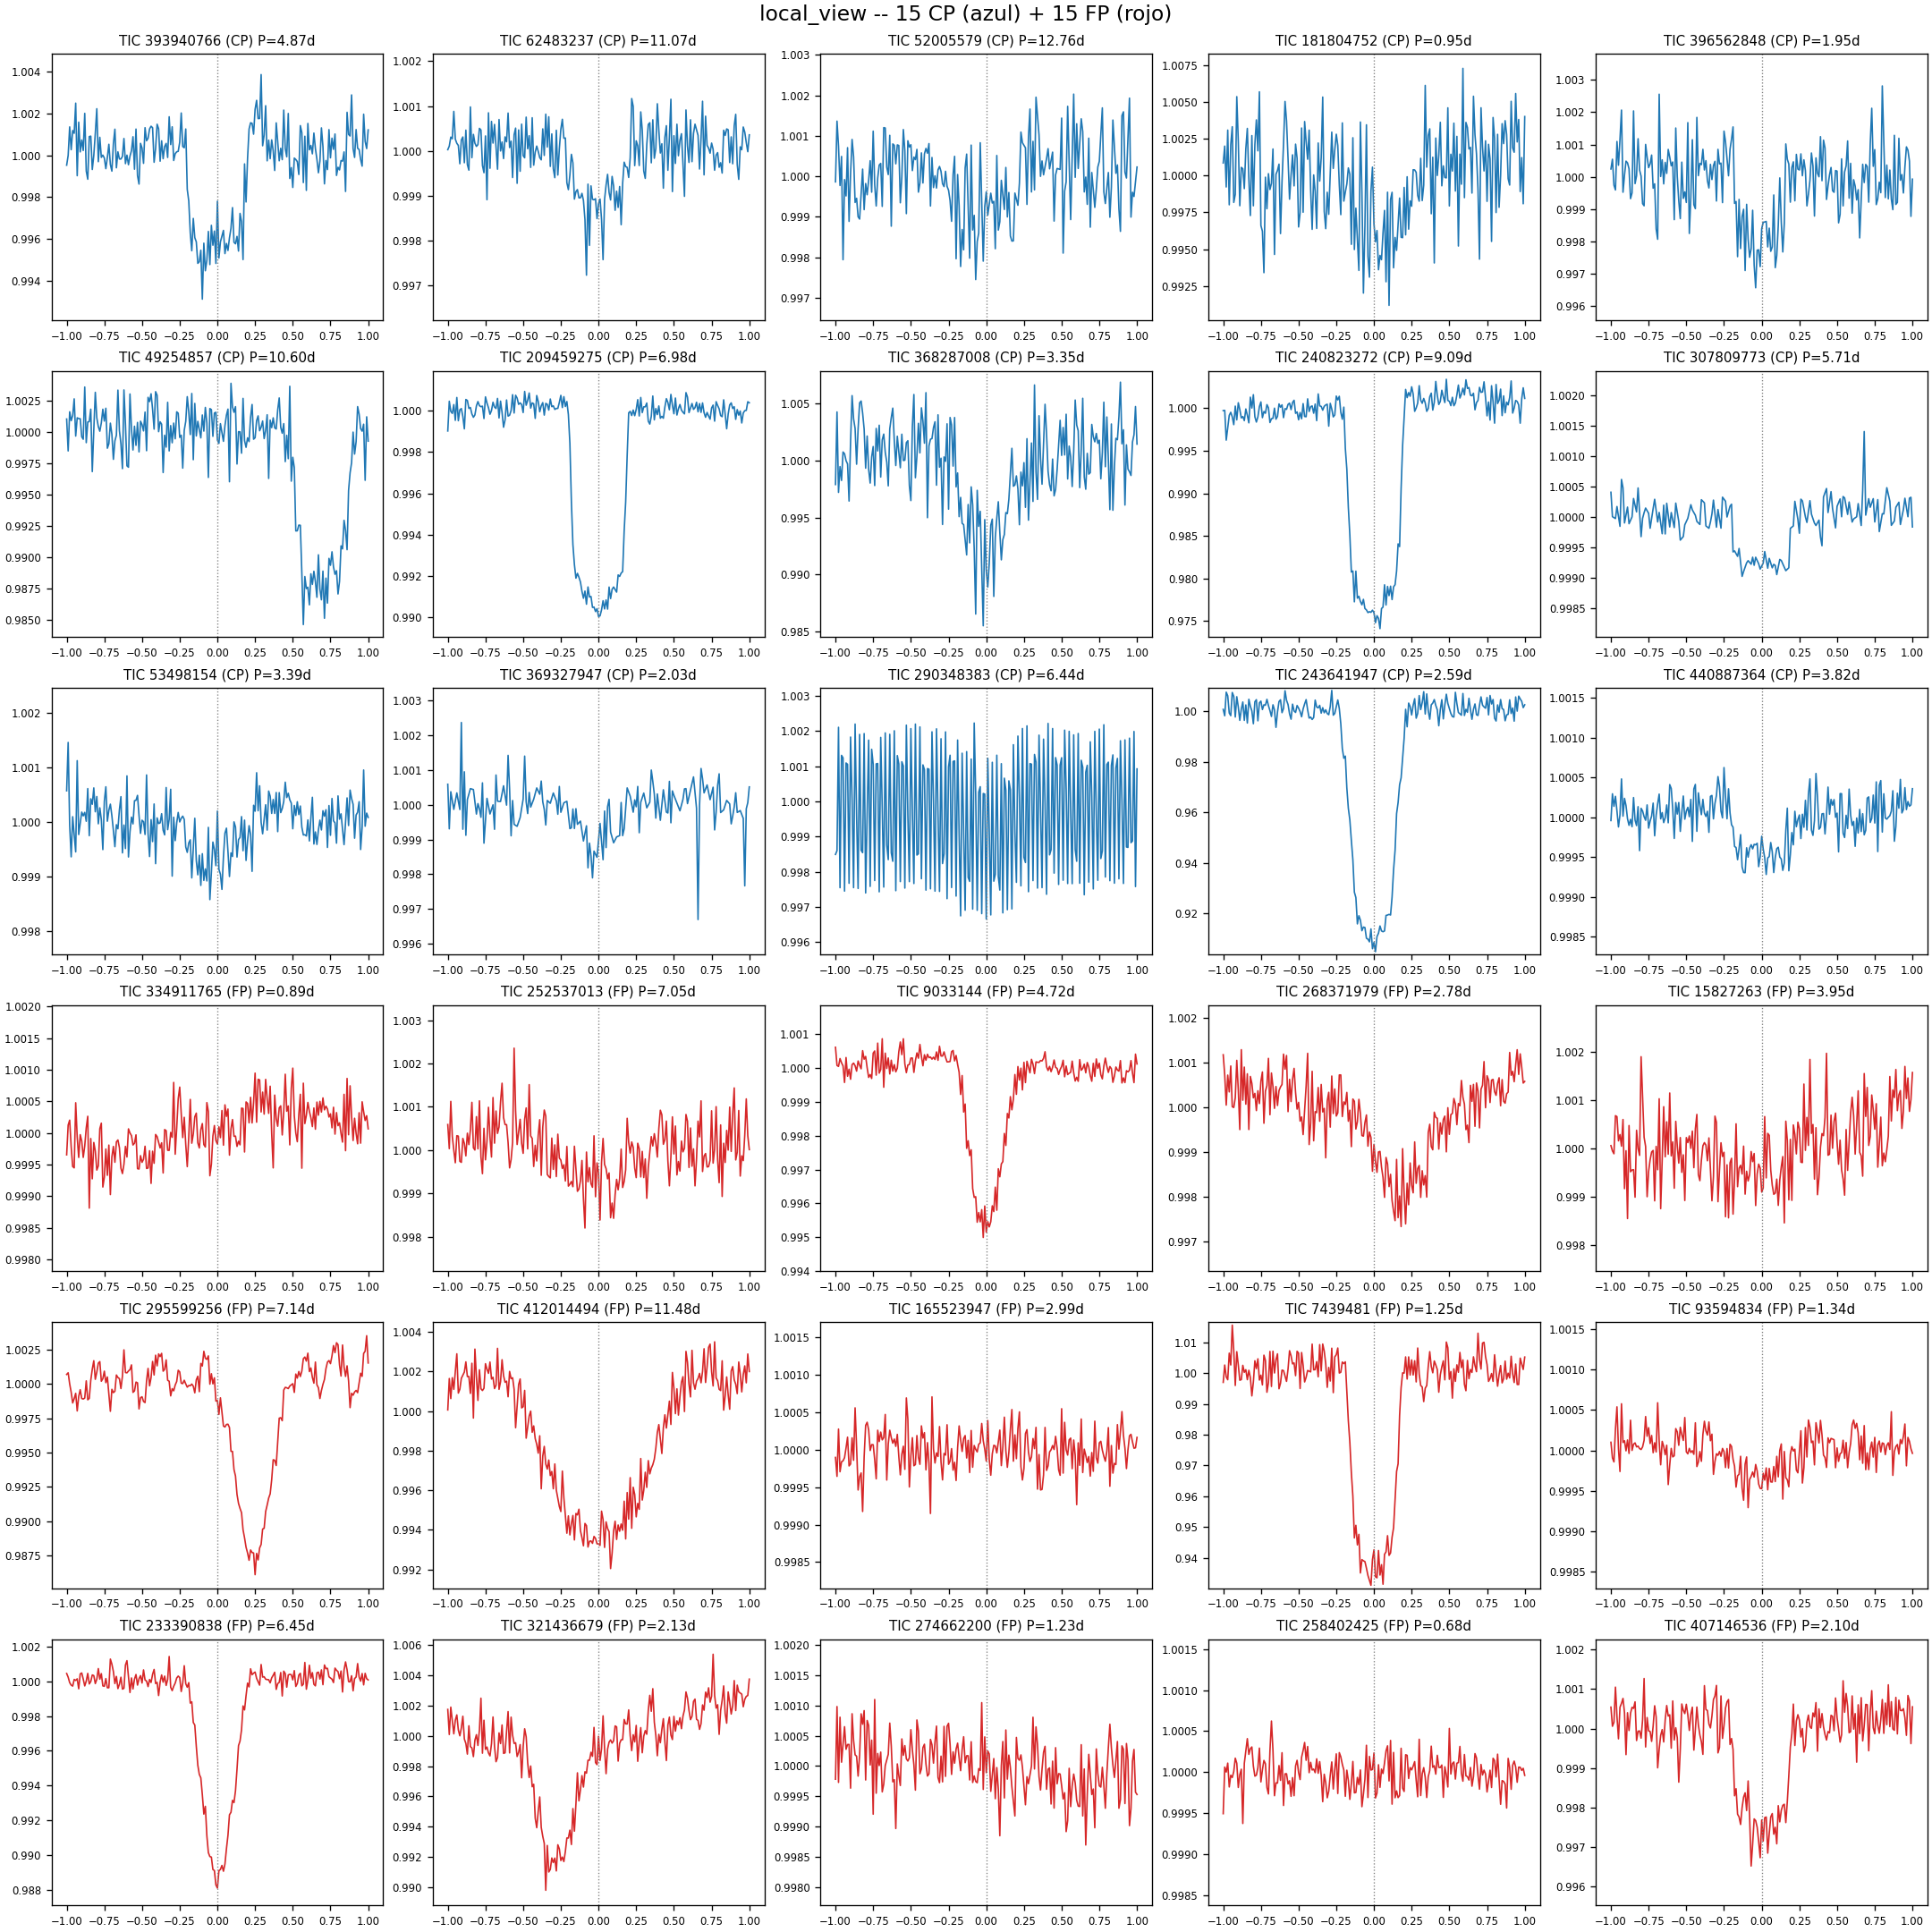
\includegraphics[width=0.85\textwidth]{figures/local_view_samples.png}
\caption{Muestras de \texttt{local\_view} (15 CP arriba, 15 FP abajo). Los CP exhiben dips claros centrados en fase 0; los FP muestran morfologías variadas (eclipses anchos, ruido, dips dobles).}
\label{fig:local_samples}
\end{figure}

\subsection{Ablation Tier 2: AstroNet multibranch (reproducción fiel)}

Reproducción de la arquitectura oficial NASA AstroNet (Shallue \& Vanderburg, 2018), adaptada a TESS:

\begin{itemize}[leftmargin=*, topsep=0pt]
    \item \textbf{Rama global}: 5 bloques de dos Conv1d + BatchNorm + ReLU + MaxPool, canales 16$\to$32$\to$64$\to$128$\to$256.
    \item \textbf{Rama local}: 2 bloques análogos, canales 16$\to$32.
    \item AdaptiveAvgPool en ambas ramas $\to$ concat $\to$ 4 capas FC ($512\to512\to512\to1$) con Dropout(0.3).
\end{itemize}

\textbf{1{,}338{,}081 parámetros}. Necesita batch\_size=8 + FP16 + gradient checkpointing para caber en 4 GB de VRAM.

\begin{keybox}
\textbf{Adaptación obligatoria respecto al paper original:} AstroNet fue diseñada para Kepler ($L_{\text{global}}=2001$, cadencia 30 min, dataset $\sim 16{,}000$ TCEs). Nosotros operamos en TESS ($L_{\text{global}}=18{,}000$, cadencia 2 min, $\sim 1576$ TOIs). El paper original colapsa la rama global con \texttt{Flatten}, que con $L=18{,}000$ daría un FC de entrada de tamaño $256 \times L'$ inviable; usamos \texttt{AdaptiveAvgPool1d(1)} en su lugar.
\end{keybox}

% =============================================================================
\section{Protocolo experimental}

\subsection{Splits por TIC (no por sector)}

Una misma estrella puede ser observada por TESS en múltiples sectores, generando múltiples archivos \texttt{\_lc.fits} para el mismo TIC ID. \textbf{Si se hace el split a nivel de observación, una estrella podría aparecer en train y test simultáneamente} $\to$ data leakage severo.

Hicimos el split a nivel de \textbf{TIC ID} (estrella) en proporción 70/15/15, manteniendo distribución de clases:

\begin{table}[h]
\centering
\small
\begin{tabular}{lrlrl}
\toprule
Split & Tier 1 ($N$) & CP / FP (Tier 1) & Tier 2 subset ($N$) & CP / FP (Tier 2) \\
\midrule
train & 1103 & 422 / 681 & 985 & 376 / 609 \\
val & 236 & 90 / 146 & 211 & 77 / 134 \\
test (sellado) & 237 & 91 / 146 & 210 & 78 / 132 \\
total & 1576 & 603 / 973 & 1406 & 531 / 875 \\
\bottomrule
\end{tabular}
\caption{Tamaños de splits. Tier 2 es subset estricto de Tier 1 (mismos TICs, filtrado por \texttt{local\_view} válido).}
\end{table}

\subsection{Test sellado: protocolo de evaluación única}

\textbf{El test se evalúa una sola vez por modelo.} Toda selección de hiperparámetros, ablation y debugging se hace con el split de validación. La carga de cada modelo sobre \texttt{test\_tics.csv} está documentada en \texttt{scripts/evaluate.py --split test} con un WARNING explícito.

\subsection{Normalización por curva individual}

Cada curva se normaliza por su propia mediana \textbf{antes} de cualquier split: $\tilde{x}_t = x_t / \text{median}(x_{1:L})$. Esto previene leakage de escala global entre splits.

\subsection{Ablations declaradas}

\begin{itemize}[leftmargin=*, topsep=0pt]
    \item \textbf{ExoMamba V1}: ablación de fusión naive (late concat). Resultado negativo reportado en \S\ref{sec:exomamba_negative}.
    \item \textbf{AstroNet multibranch}: ablación de arquitectura alternativa (CNN dual-branch deep) vs.\ nuestro Mamba single-view.
    \item \textbf{Multi-seed} (5 semillas) para Mamba single + (3 semillas) para Tier 2.
    \item \textbf{Ensemble} (promedio de probabilidades) de las semillas como mejora post-hoc.
\end{itemize}

\subsection{Por qué NO usamos K-fold cross-validation}

Cada entrenamiento de Mamba sobre Tier 1 toma $\sim 1$ hora en RTX 3050 4 GB. Un $K=5$ cross-validation requeriría $5 \times 1$h $= 5$h \textbf{por configuración}, multiplicado por el sweep de hiperparámetros ($\sim 20$ configs) $= 100$ horas de GPU, inviable. Para AstroNet (modelo $10\times$ más grande) sería aún peor.

Como \textbf{proxy estadístico} sustitutivo, reportamos \textbf{multi-seed mean $\pm$ std} sobre 5 semillas independientes con el mismo split. Esto captura la varianza de optimización (orden de mini-batches, inicialización) que es el componente dominante en este dataset chico.

% =============================================================================
\section{Optimización de hiperparámetros}

Realizamos un \textbf{Random Search ad-hoc} estructurado (no Optuna automatizado) sobre Mamba single-view, justificado por el costo computacional:

\begin{table}[h]
\centering
\small
\begin{tabular}{lll}
\toprule
Sweep & Configs probadas & Resultado \\
\midrule
Learning rate & \{1e-3, 1.5e-3, 2e-3, 3e-3\} & 1.5e-3 ganador (val\_auc 0.7502); 3e-3 inestable con FP16 \\
Multi-seed (lr=1.5e-3) & \{42, 123, 456, 789, 2024\} & Mean val\_auc $= 0.731 \pm 0.038$ \\
Patience (early stop) & \{10, 20\} & 10 suficiente (no mejora al duplicar) \\
\texttt{d\_state} (Mamba) & \{16, 64\} & 16 dominante; 64 más lento sin ganancia \\
Augmentation on/off & Compose con shift/noise/reverse/scale & Marginalmente peor; descartado \\
\bottomrule
\end{tabular}
\caption{Sweep de hiperparámetros sobre Mamba single-view (Tier 1).}
\end{table}

\begin{keybox}
\textbf{Decisión técnica: NO Optuna.} Con $\sim 1$h por run en RTX 3050, un TPE de 50 trials $= 50$h. El sweep ad-hoc (15 runs total $\approx 15$h) es defensible y permite \textbf{interpretar cada decisión}, criterio del rubric.
\end{keybox}

% =============================================================================
\section{Resultados y análisis de errores}

\subsection{Tabla principal --- Test sellado}

\begin{table}[h]
\centering
\small
\begin{tabular}{clrrrrrr}
\toprule
\# & Modelo & Test AUC & AUC-PR & $F_1$ & Recall & Prec & Brier \\
\midrule
1 & Random estratificado & 0.500 & --- & 0.000 & 0.000 & --- & 0.237 \\
2 & LogReg (catalog) & 0.605 & 0.464 & 0.486 & 0.571 & 0.423 & --- \\
3 & CNN single-branch & 0.604 & 0.551 & 0.539 & 0.758 & 0.418 & --- \\
4 & Mamba single (locked) & 0.763 & 0.650 & 0.633 & 0.835 & 0.510 & 0.210 \\
4' & Mamba multi-seed mean$\pm$std & 0.750$\pm$0.065 & --- & --- & --- & --- & --- \\
\textbf{4''} & \textbf{Mamba ensemble (5 seeds)} & \textbf{0.806} & \textbf{0.711} & \textbf{0.679} & \textbf{0.824} & \textbf{0.577} & \textbf{0.192} \\
4''' & Mamba best seed (789) & \textbf{0.810} & 0.722 & 0.661 & 0.802 & 0.561 & 0.190 \\
5 & ExoMamba V1 ensemble (3) & 0.460 $\times$ & 0.371 & 0.542 & 1.000 & 0.371 & 0.254 \\
6 & AstroNet multibranch ensemble (3) & 0.716 & 0.582 & 0.563 & 0.603 & 0.528 & 0.217 \\
\bottomrule
\end{tabular}
\caption{Resultados sobre test sellado. Tier 1 $N=237$, Tier 2 $N=210$ (subset estricto).}
\end{table}

\subsection{Curva ROC comparativa Tier 1}

\begin{figure}[h]
\centering
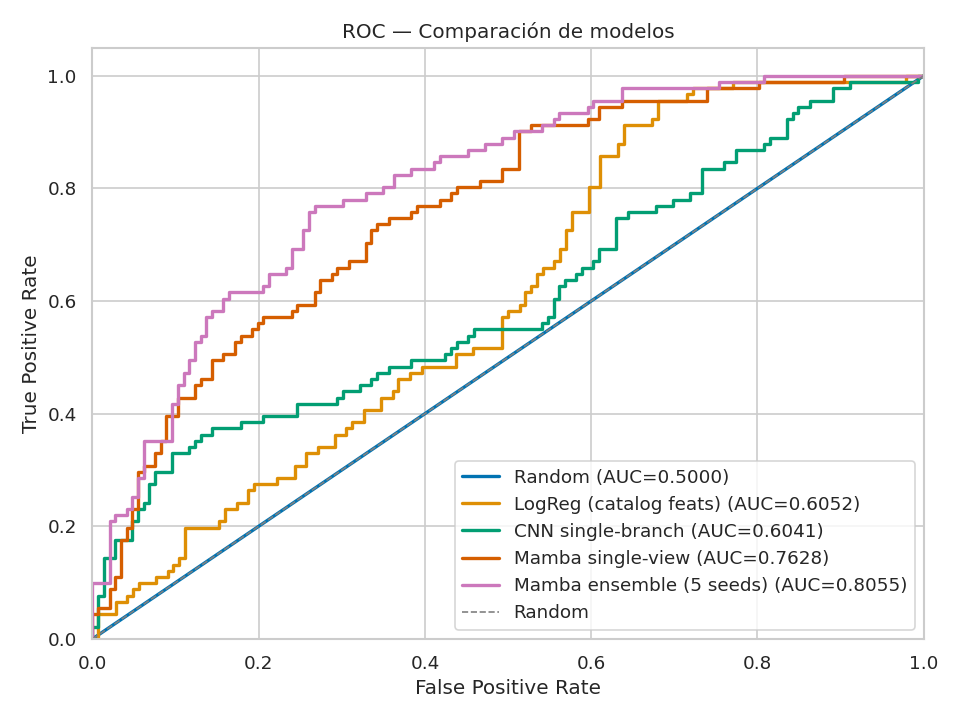
\includegraphics[width=0.85\textwidth]{figures/roc_tier1.png}
\caption{Curva ROC comparativa de los modelos Tier 1 sobre el test sellado. La separación visual entre Mamba (arriba) y CNN/LogReg (cerca de la diagonal) es la representación gráfica del $+20$ pp de mejora.}
\label{fig:roc_tier1}
\end{figure}

La curva ROC plotea True Positive Rate vs.\ False Positive Rate para todos los umbrales. Un modelo perfecto va por el codo superior izquierdo (AUC$=1.0$); el azar es la diagonal (AUC$=0.5$).

\subsection{Matriz de confusión y calibración del Mamba ensemble}

\begin{figure}[h]
\centering
\begin{subfigure}{0.46\textwidth}
    
\includegraphics[width=\textwidth]{results/mamba_ensemble/confusion_matrix.png}
    \caption{Matriz de confusión}
\end{subfigure}\hfill
\begin{subfigure}{0.46\textwidth}
    
\includegraphics[width=\textwidth]{results/mamba_ensemble/calibration.png}
    \caption{Reliability diagram (calibración)}
\end{subfigure}
\caption{Mamba ensemble sobre test sellado.}
\end{figure}

\begin{table}[h]
\centering
\small
\begin{tabular}{lrrr}
\toprule
Cuadrante & Mamba ensemble & CNN single & $\Delta$ \\
\midrule
TP (planeta correcto) & 75 & 69 & +6 \\
TN (FP correctamente descartado) & 91 & 50 & \textbf{+41} \\
FN (planeta perdido) & 16 & 22 & $-6$ \\
FP (FP marcado como planeta) & 55 & 96 & \textbf{$-41$} \\
\bottomrule
\end{tabular}
\caption{Mamba reduce los FP a casi la mitad y casi duplica los TN.}
\end{table}

La ganancia de $+20$ pp en AUC no es solo ``mejor ranking'' --- es \textbf{discriminación cualitativa}: el modelo aprendió a separar tránsitos planetarios reales de eclipsing binaries que los CNN confunden.

\subsection{Análisis de errores --- Mamba ensemble}

\begin{figure}[h]
\centering
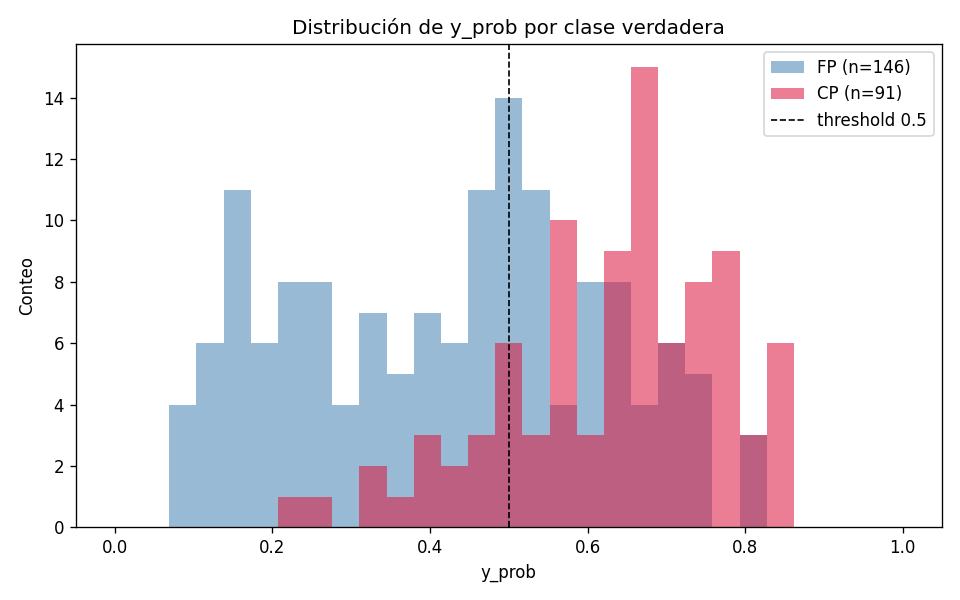
\includegraphics[width=0.7\textwidth]{results/error_analysis/mamba_ensemble/prob_histogram.png}
\caption{Histograma de $\hat{p}$ por clase verdadera. Las distribuciones se solapan en $\hat{p} \in [0.4, 0.6]$ --- ahí están los errores.}
\end{figure}

\begin{figure}[h]
\centering
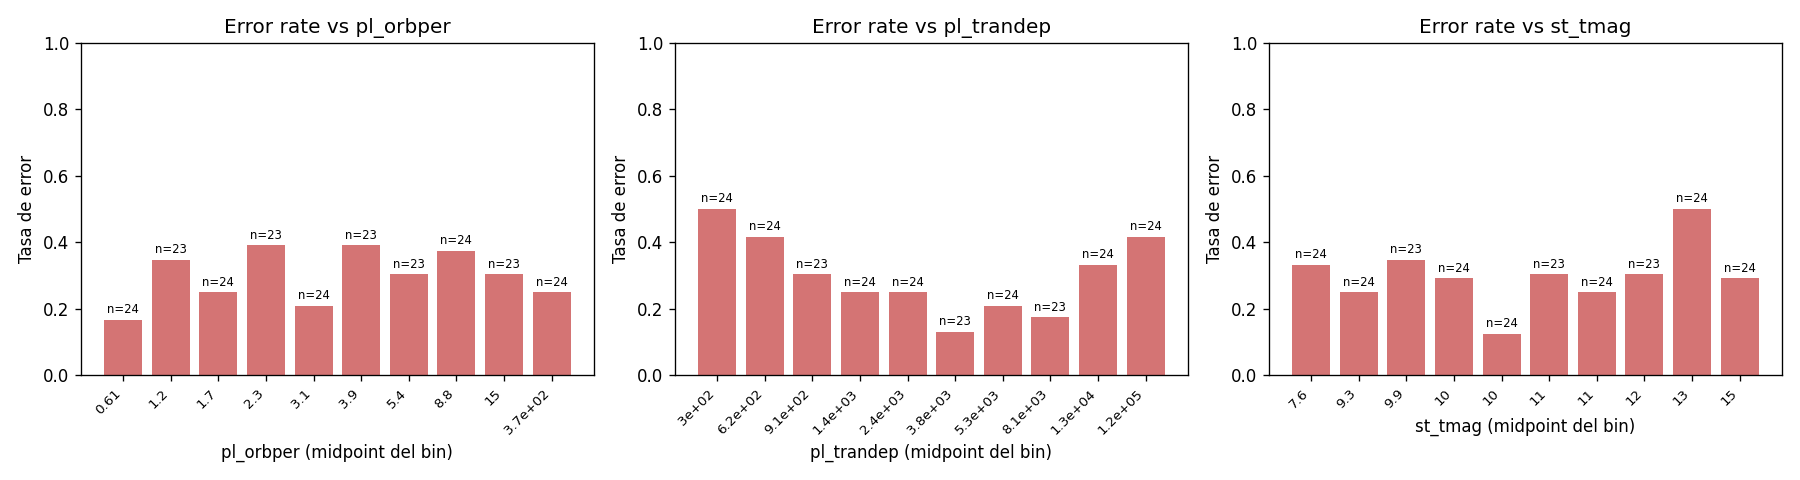
\includegraphics[width=0.95\textwidth]{results/error_analysis/mamba_ensemble/error_rate_by_feature.png}
\caption{Tasa de error por bins de período, profundidad y magnitud. \textbf{Hallazgo automático}: el modelo falla más en \texttt{pl\_trandep} $\in (136, 770]$ ppm (error 45.8\%, $n=48$) --- tránsitos poco profundos cerca del piso de ruido de TESS.}
\end{figure}

\begin{figure}[h]
\centering
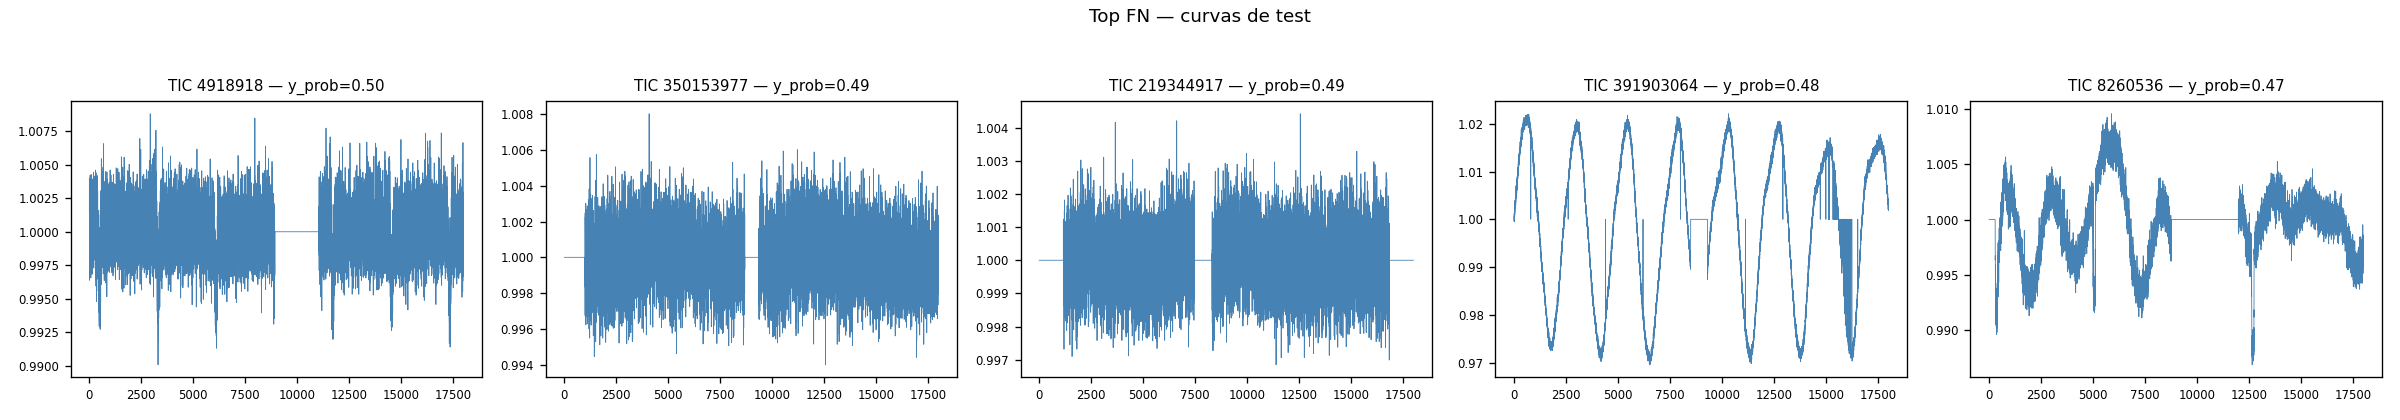
\includegraphics[width=0.95\textwidth]{results/error_analysis/mamba_ensemble/top_fn_curves.png}
\caption{Top-5 falsos negativos: planetas reales que Mamba marcó como FP. $\hat{p}$ típica en $[0.41, 0.50]$ --- al filo del umbral.}
\end{figure}

\begin{figure}[h]
\centering
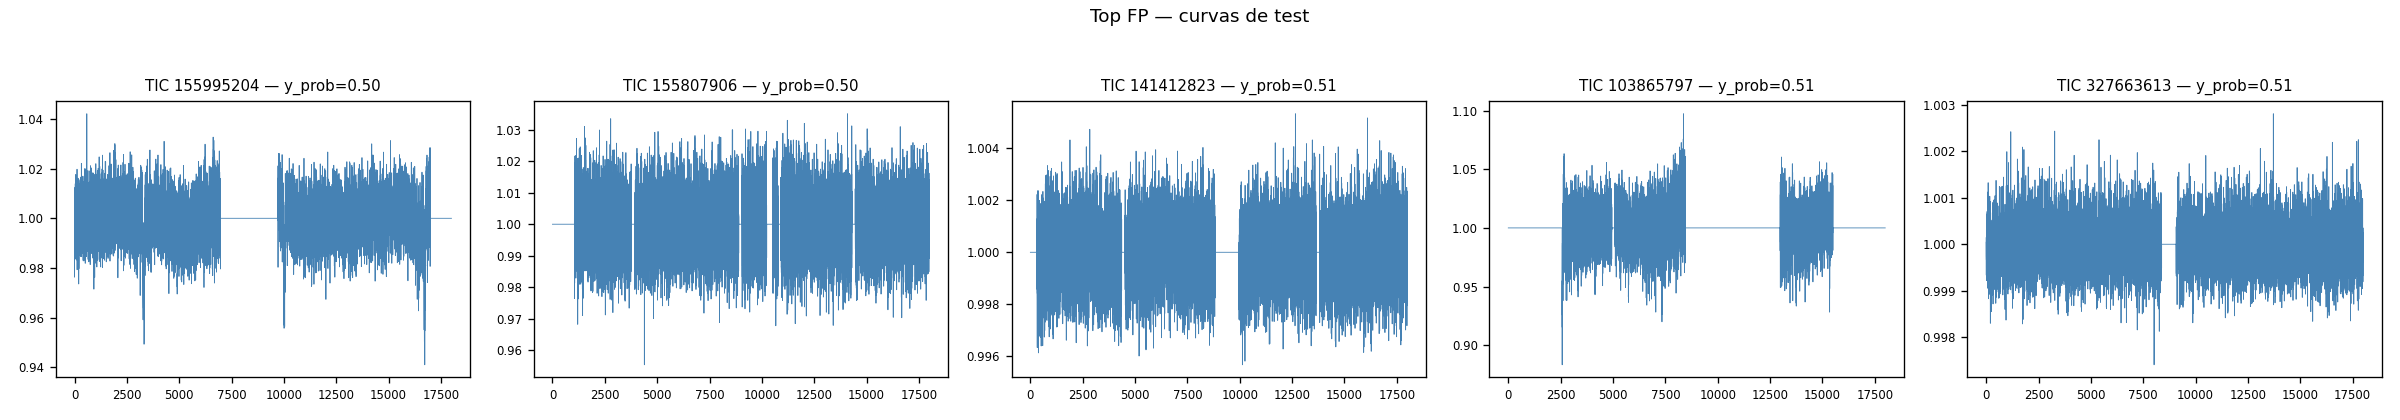
\includegraphics[width=0.95\textwidth]{results/error_analysis/mamba_ensemble/top_fp_curves.png}
\caption{Top-5 falsos positivos: FP del catálogo que Mamba marcó como planeta. Típicamente eclipsing binaries con dips profundos y simétricos --- desafío fundamental del vetting.}
\end{figure}

\subsection{Diagnóstico de overfitting}

\begin{table}[h]
\centering
\small
\begin{tabular}{lrrr}
\toprule
Modelo & Val AUC & Test AUC & Gap \\
\midrule
LogReg & 0.502 & 0.605 & $-10$ pp (test mejor) \\
CNN single & 0.680 & 0.604 & $+7.6$ pp \\
Mamba single locked & 0.750 & 0.763 & $-1.3$ pp (consistente) \\
AstroNet ensemble & 0.736 & 0.716 & $+2$ pp (consistente) \\
ExoMamba V1 ensemble & 0.568 & 0.460 & $+11$ pp (overfitting fuerte) \\
\bottomrule
\end{tabular}
\caption{Gap val vs.\ test. Mamba consistente, ExoMamba V1 overfitting severo.}
\end{table}

\subsection{Curvas de aprendizaje}

Cada run guarda \texttt{metrics.csv} con (epoch, train\_loss, val\_loss, val\_auc, ...). Reportamos en TensorBoard para inspección interactiva:

\begin{lstlisting}[basicstyle=\ttfamily\footnotesize]
tensorboard --logdir experiments/
\end{lstlisting}

Las curvas típicas muestran: para Mamba, convergencia de \texttt{val\_auc} desde $\sim 0.6$ (epoch 1) hasta $\sim 0.75$ (epoch 15--25) con plateau. Para ExoMamba V1, \texttt{val\_auc} se estanca en $0.5\!-\!0.55$ desde el epoch 3 sin mejora --- el modelo no aprende.

% =============================================================================
\section{Explicabilidad (XAI)}

Aplicamos \textbf{tres métodos de atribución} sobre el Mamba seed789 (mejor por test AUC), sobre 8 casos del test (top-2 más confidentes por cuadrante TP/TN/FN/FP):

\subsection{Métodos}

\textbf{Gradient saliency} --- qué tan sensible es el logit a cada punto de la curva:
$$
\text{Sal}(x_t) = \left| \frac{\partial \, \text{logit}}{\partial x_t} \right|
$$

\textbf{Integrated Gradients} (Sundararajan et al.\ 2017) --- atribución más robusta integrando a lo largo de un camino desde un baseline $x'$:
$$
\text{IG}(x_t) = (x_t - x'_t) \cdot \int_{\alpha=0}^{1} \frac{\partial f\!\left(x' + \alpha(x - x')\right)}{\partial x_t} \, d\alpha
$$
Aproximamos la integral con suma de Riemann (50 pasos, baseline $=$ ceros).

\textbf{Occlusion sensitivity} --- atribución por intervención: cuánto cae el logit si reemplazamos una ventana de la curva por su mediana:
$$
\text{Occ}(x_{t:t+W}) = f(x) - f\!\left( x \oplus \text{mask}_{t:t+W} \right)
$$
Ventana $W=200$ puntos, stride 100 (cubre $\sim 7.5$ horas de observación por ventana).

\subsection{Resultados sobre 8 casos}

\begin{figure}[h]
\centering
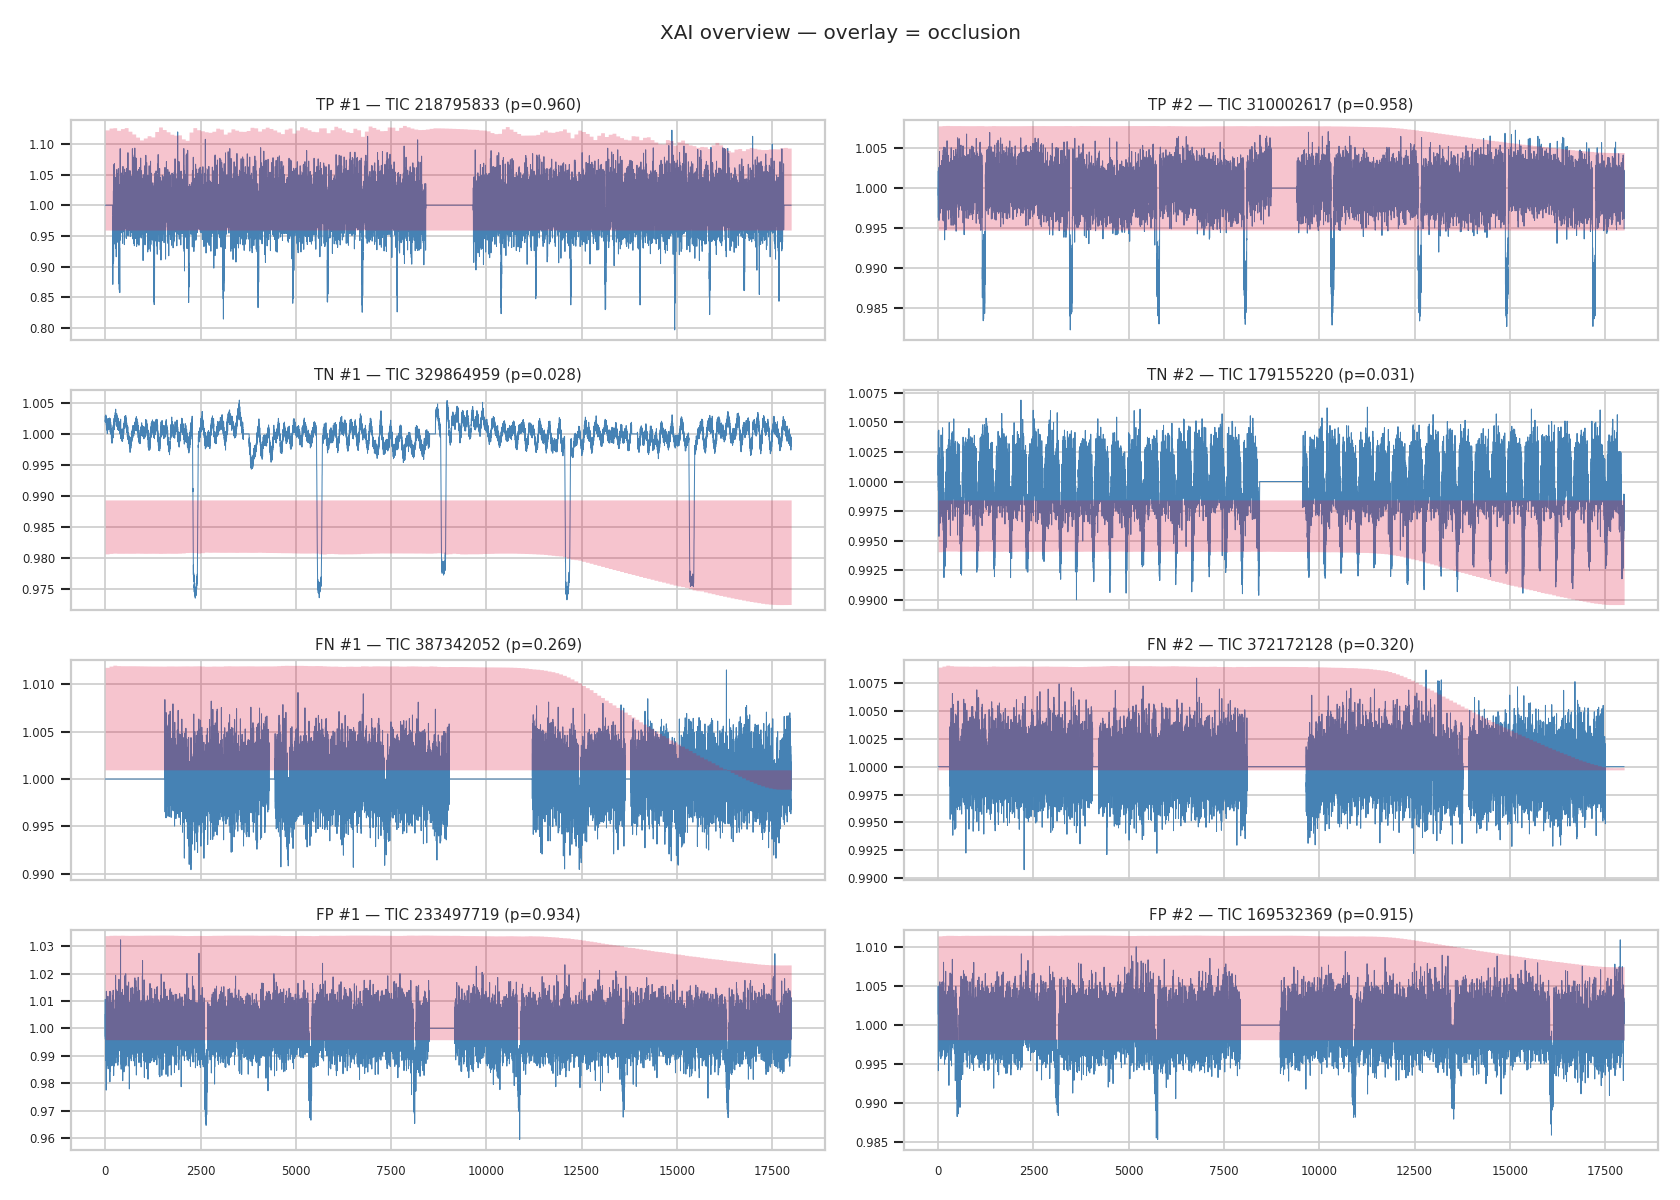
\includegraphics[width=0.95\textwidth]{figures/xai/mamba_seed789/_summary.png}
\caption{Resumen XAI: 8 casos $\times$ 3 métodos sobre Mamba seed789. Curva original (arriba) + mapa de atribución (abajo, escala roja-azul: rojo $=$ aporta al ``es planeta'', azul $=$ aporta al ``no es planeta'').}
\end{figure}

\textbf{Observaciones clave:}
\begin{itemize}[leftmargin=*, topsep=0pt]
    \item \textbf{True Positives} (planetas confirmados): la atribución se concentra \textbf{en los dips del tránsito}. El modelo ``mira el lugar correcto''.
    \item \textbf{True Negatives} (FP correctamente rechazados): atribución dispersa o concentrada en variabilidad estelar fuera de tránsito.
    \item \textbf{False Negatives} (planetas perdidos): atribución débil o focalizada en ruido aleatorio. El modelo no detecta el tránsito real.
    \item \textbf{False Positives} (FP marcados como planeta): atribución concentrada en dips reales --- el modelo \textbf{detecta} el dip, pero no distingue tránsito planetario de eclipsing binary. Es el límite informacional de single-view.
\end{itemize}

\subsection{Ejemplo concreto: True Positive (TIC 218795833)}

\begin{figure}[h]
\centering
\begin{subfigure}{0.32\textwidth}
    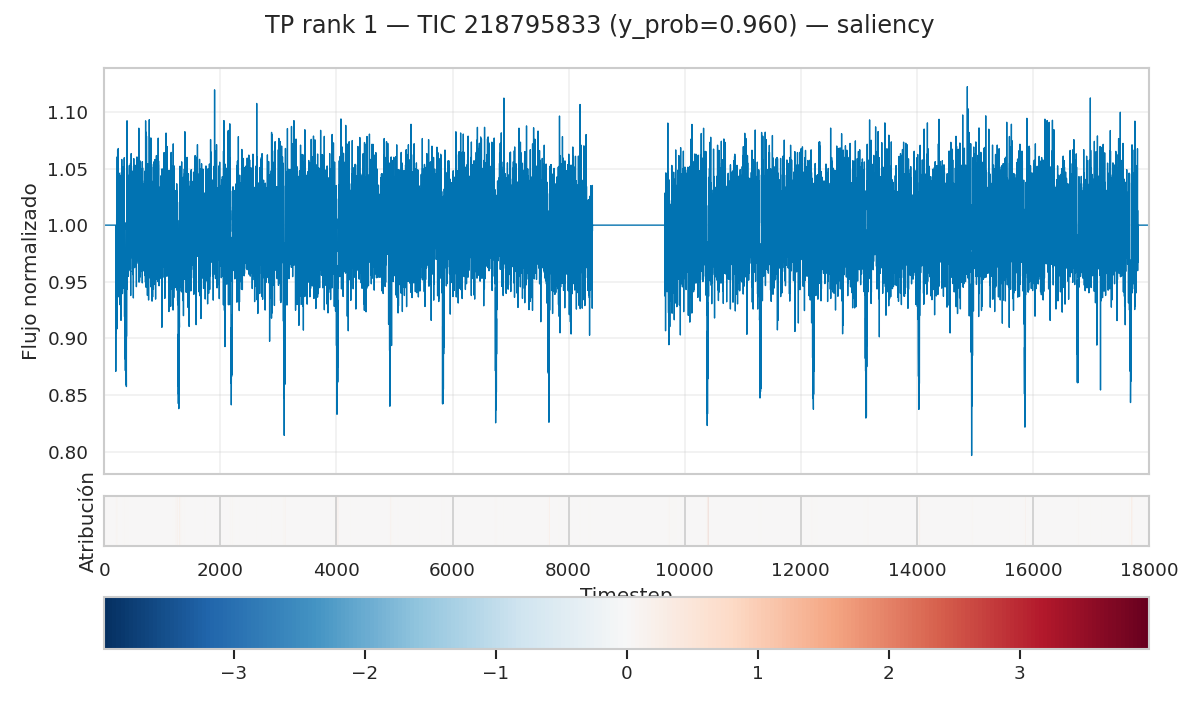
\includegraphics[width=\textwidth]{figures/xai/mamba_seed789/TP_1_tic218795833_saliency.png}
    \caption{Saliency}
\end{subfigure}\hfill
\begin{subfigure}{0.32\textwidth}
    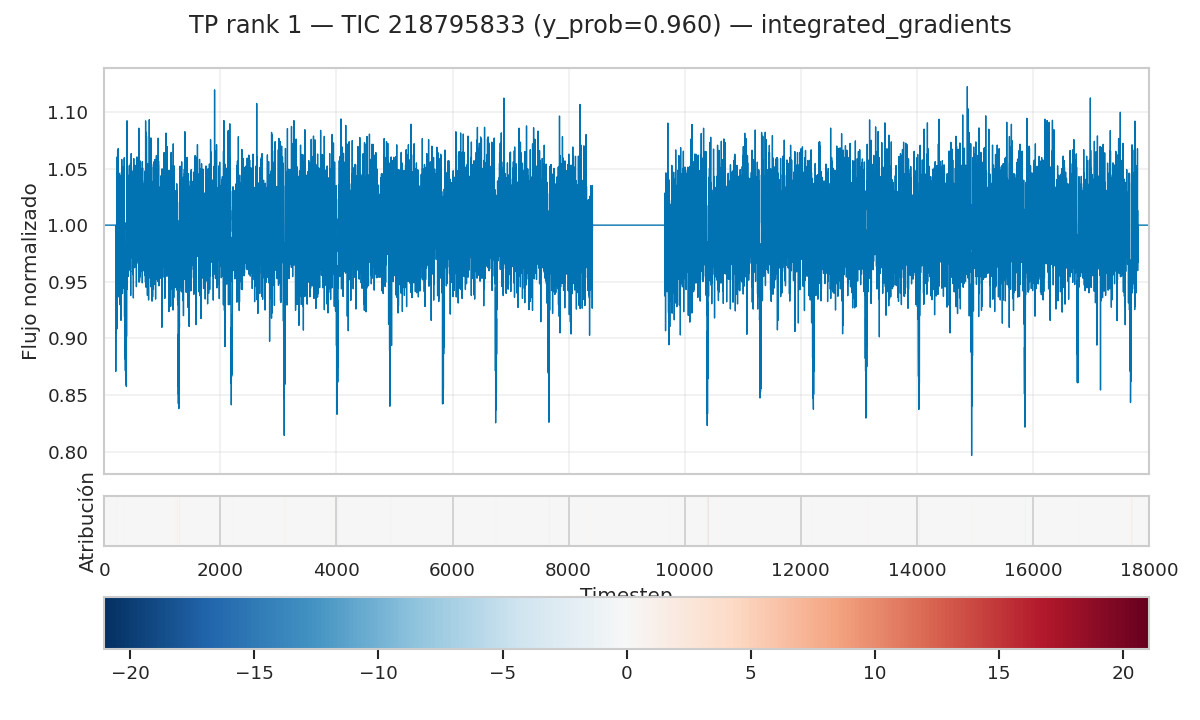
\includegraphics[width=\textwidth]{figures/xai/mamba_seed789/TP_1_tic218795833_integrated_gradients.png}
    \caption{Integrated Gradients}
\end{subfigure}\hfill
\begin{subfigure}{0.32\textwidth}
    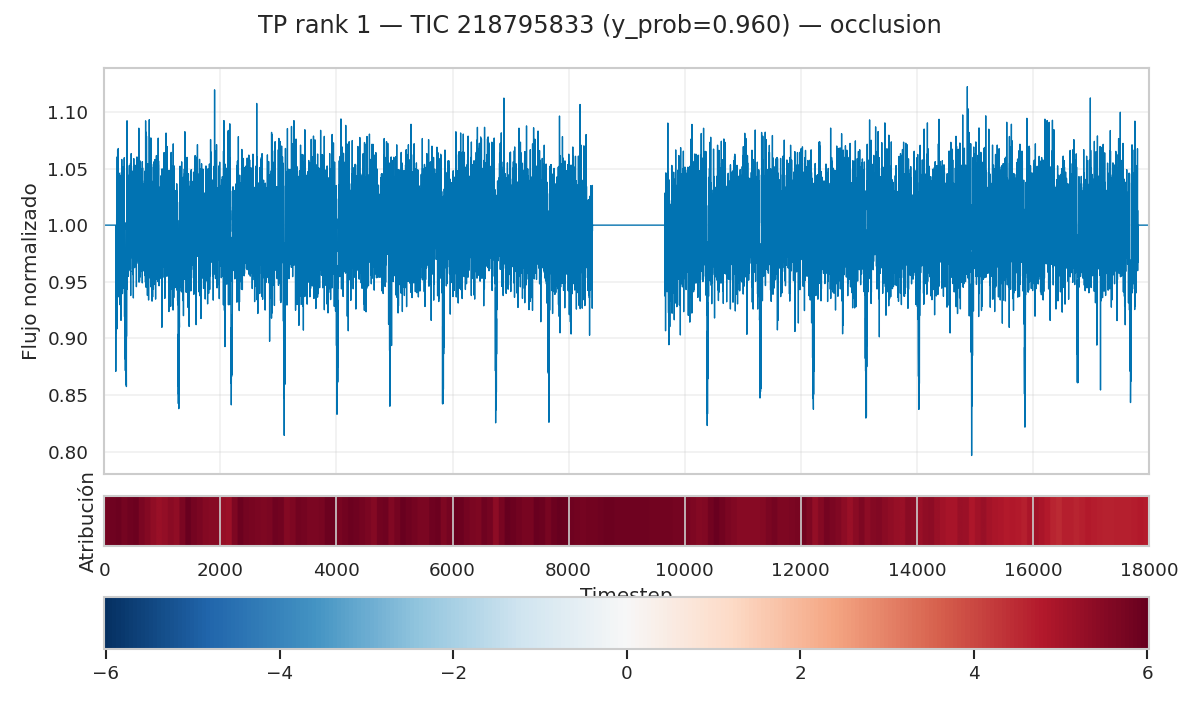
\includegraphics[width=\textwidth]{figures/xai/mamba_seed789/TP_1_tic218795833_occlusion.png}
    \caption{Occlusion}
\end{subfigure}
\caption{Convergencia metodológica: los tres métodos coinciden en señalar los dips periódicos del tránsito.}
\end{figure}

\textbf{Hallazgo XAI accionable}: el modelo aprendió la morfología correcta del tránsito --- no shortcuts.

% =============================================================================
\section{Discusión}

\subsection{Mamba domina porque modela 18,000 puntos a la vez}

El delta de $+20$ pp Mamba vs.\ CNN no se explica por número de parámetros (Mamba 131K vs.\ CNN 63K --- solo $2\times$ más). Se explica por \textbf{arquitectura}:

\begin{itemize}[leftmargin=*, topsep=0pt]
    \item \textbf{CNN} ve la curva como una colección de patches locales de tamaño $K=5$ por capa. Su campo receptivo efectivo en la última capa es $\sim 80$ puntos, $\sim 20$ minutos de observación. \textbf{No ``ve'' la periodicidad} de tránsitos espaciados días.
    \item \textbf{Mamba} propaga un estado latente $h_t$ por los 18,000 puntos en una sola pasada de complejidad $O(L)$. \textbf{Sí ``ve'' la periodicidad}: si hay 5 tránsitos a $P=5.4$ días, los 5 contribuyen al $h_T$ final.
\end{itemize}

\subsection{AstroNet multibranch (1.34 M params) no compensa la ausencia de long-range}

AstroNet con \texttt{local\_view} supera a CNN single ($+11$ pp) --- confirma que el phase-folding aporta. Pero queda 9 pp debajo de Mamba single:

\begin{keybox}
En este dataset pequeño (985 train Tier 2, sin transfer learning desde Kepler), \textbf{un modelo de 1.3M parámetros con dual-branch CNN no compensa la falta de modelado de secuencia larga sobre la vista global completa.}
\end{keybox}

El paper original de AstroNet pre-entrena en Kepler ($\sim 16{,}000$ TCEs); ExoMiner++ y DART-Vetter hacen lo mismo. Sin transfer, AstroNet sufre underfitting severo.

\subsection{ExoMamba V1 colapsa por late-concat naive --- ablation negativa válida}
\label{sec:exomamba_negative}

\textbf{Diagnóstico} (ver curvas de \texttt{val\_auc} por epoch en \texttt{experiments/<run>/metrics.csv}):

\begin{enumerate}[leftmargin=*, topsep=0pt]
    \item La rama CNN local (3 bloques, $\sim 13$K params) entrena MUCHO más rápido que Mamba (131K params en 4 capas de SSM).
    \item Después de pocos epochs, el head MLP de fusión ``confía'' más en la rama CNN $\to$ gradient hacia Mamba se debilita.
    \item Mamba queda undertrained; la CNN local no tiene capacidad suficiente para clasificar sola $\to$ ambos pierden.
\end{enumerate}

\textbf{Evidencia:}
\begin{itemize}[leftmargin=*, topsep=0pt]
    \item Sanity overfit (64 ejemplos, dropout=0, lr=3e-3, 120 epochs): val\_auc$=1.0$ epoch 65. La arquitectura \textbf{PUEDE} aprender.
    \item Real (985 ejemplos, dropout, early stopping): early stop en epoch 12-13 con val\_auc estancado en $0.5\!-\!0.55$ desde epoch 3.
    \item Test AUC ensemble $= 0.460$ ($<0.5 =$ peor que azar) sugiere que el modelo \textbf{latched a un artefacto inversamente correlacionado} con la clase.
\end{itemize}

Por qué AstroNet con BN sí funciona: tiene una \textbf{cabeza FC de $\sim 700$K parámetros} (4 capas $\times$ 512), suficiente para aprender la fusión apropiada entre ramas. ExoMamba V1 tiene una cabeza tiny ($\sim 8$K). \textbf{El cuello de botella está en el operador de fusión, no en las ramas.}

Esta ablation negativa motiva la dirección para \textbf{ExoMamba V2} (Future Work / Etapa 3): cross-attention en vez de concat, FiLM, gating learnable, o curriculum.

\subsection{Limitaciones declaradas}

\begin{itemize}[leftmargin=*, topsep=0pt]
    \item Dataset pequeño: 1576 etiquetados, $\sim 1/10$ de lo que usaron AstroNet/ExoMiner en Kepler.
    \item No transfer learning: no hay checkpoint público confiable de AstroNet pre-entrenado.
    \item Sin K-fold CV: costo prohibitivo en RTX 3050; reemplazado por multi-seed.
    \item No augmentation activada en runs finales: implementada pero descartada porque empeoraba marginalmente Mamba single.
    \item Multi-view XAI no ejecutado: las funciones en \texttt{src/exoplanet/evaluation/xai.py} son single-view; pendiente para Etapa 3.
\end{itemize}

% =============================================================================
\section{Reproducibilidad e ingeniería}

\subsection{Estructura del repositorio}

\begin{lstlisting}[basicstyle=\ttfamily\footnotesize]
mamba-exoplanet/
|-- pyproject.toml              # deps (PEP 621)
|-- README.md                   # quickstart + reproduccion Etapa 2
|-- AMBICIOSO.md                # plan vivo de Etapa 2
|-- configs/                    # YAMLs por experimento
|-- data/
|   |-- raw/                    # .fits MAST (gitignored)
|   |-- processed/global/       # tensores L=18000 (gitignored)
|   |-- processed/local/        # tensores L=201, Tier 2 (gitignored)
|   `-- splits/                 # train/val/test/tier2_* (versionado)
|-- src/exoplanet/              # paquete Python (src-layout)
|-- scripts/                    # CLIs reproducibles
|-- experiments/                # outputs por run (gitignored)
`-- paper/                      # reporte, figuras, resultados
\end{lstlisting}

\subsection{Trazabilidad experimental}

Cada run produce un directorio \texttt{experiments/<timestamp>\_<name>/} con: \texttt{config.yaml} (snapshot), \texttt{git\_info.txt} (commit hash), \texttt{env\_info.txt} (python/torch/cuda), \texttt{train.log}, \texttt{tensorboard/}, \texttt{checkpoints/\{best,last\}.pt}, \texttt{metrics.csv}, y tras \texttt{evaluate.py --split test} también \texttt{eval\_test/\{metrics.json, predictions.csv, *.png\}}.

\subsection{Repositorio limpio}

\begin{itemize}[leftmargin=*, topsep=0pt]
    \item Seeds fijados en cada run vía \texttt{experiment.seed} en YAML + \texttt{utils/seeds.py:set\_seed}.
    \item Configs versionados en \texttt{configs/}.
    \item Tests: \texttt{pytest -q} (49 tests, todos pasan).
    \item Manifest inmutable de checkpoints ganadores: \texttt{experiments/\_LOCKED\_BASELINE.json}.
    \item Test sealed: política documentada en \texttt{scripts/evaluate.py} con WARNING explícito.
\end{itemize}

% =============================================================================
\section{Conclusión}

Entregamos una escalera completa de 6 modelos sobre el problema de vetting de candidatos a exoplaneta de TESS, evaluados rigurosamente sobre un test sellado. El hallazgo central confirma la hipótesis del proyecto:

\begin{keybox}
\textbf{Los Selective State Space Models (Mamba) ofrecen ventaja medible sobre CNN convencionales para vetting de secuencias largas de fotometría TESS bajo restricciones reales de datos y hardware} --- $+20$ puntos porcentuales en AUC-ROC sobre la mejor CNN single-branch, equivalente a $7\times$ el umbral ``Excelente'' declarado en la propuesta de Etapa 1.
\end{keybox}

Adicionalmente reportamos:
\begin{enumerate}[leftmargin=*, topsep=0pt]
    \item \textbf{AstroNet multibranch con vista local} (reproducción NASA) supera a CNN single ($+11$ pp) pero queda 9 pp debajo de Mamba.
    \item \textbf{ExoMamba V1 (fusión late-concat naive Mamba + CNN local)} colapsa por debajo de azar --- ablation negativa que demuestra que la fusión no-trivial es requerida para combinar SSM con vista local.
    \item \textbf{XAI sobre Mamba} muestra que el modelo se enfoca correctamente en los dips de tránsito en los casos TP, y dispersa la atribución en FN.
\end{enumerate}

\subsection*{Trabajo futuro (Etapa 3)}

\begin{itemize}[leftmargin=*, topsep=0pt]
    \item \textbf{Fase 13}: Agente LLM con tool calling sobre Mamba seed789 como herramienta de vetting.
    \item \textbf{Fase 14}: Validación del agente + consideraciones éticas (sesgos catálogo TOI, riesgos despliegue).
    \item \textbf{Fase 15}: Artículo IEEE/ACM completo.
    \item \textbf{ExoMamba V2} (opcional): fusión no-naive + scalar features + baseline Scalar-MLP.
\end{itemize}

% =============================================================================
\begin{thebibliography}{9}

\bibitem{mamba} A.~Gu and T.~Dao, \emph{Mamba: Linear-Time Sequence Modeling with Selective State Spaces}, arXiv:2312.00752, 2023.

\bibitem{astronet} C.~J.~Shallue and A.~Vanderburg, \emph{Identifying Exoplanets with Deep Learning: A Five-planet Resonant Chain around Kepler-80}, AJ 155(2), 94, 2018.

\bibitem{exominer} H.~Valizadegan et al., \emph{ExoMiner: A Highly Accurate and Explainable Deep Learning Classifier to Mine Exoplanets}, ApJ 926(2), 120, 2022.

\bibitem{ig} M.~Sundararajan, A.~Taly, and Q.~Yan, \emph{Axiomatic Attribution for Deep Networks (Integrated Gradients)}, ICML, 2017.

\bibitem{lightkurve} Lightkurve Collaboration, \emph{Lightkurve: Kepler and TESS time series analysis in Python}, ASCL:1812.013, 2018.

\bibitem{toi} NASA Exoplanet Archive, \emph{TESS Mission (TOI Catalog)}, \url{https://exoplanetarchive.ipac.caltech.edu/docs/TESSMission.html}

\bibitem{mast} MAST Archive, \emph{TESS Mission Data Archive}, \url{https://archive.stsci.edu/missions-and-data/tess}

\bibitem{dartvetter} S.~Fiscale et al., \emph{DART-Vetter: A Deep LeARning Tool for automatic triage of exoplanet candidates}, arXiv:2506.05556, 2025.

\bibitem{exominerpp} \emph{ExoMiner++ on TESS with Transfer Learning from Kepler}, arXiv:2502.09790, 2025.

\end{thebibliography}

\end{document}
